\chapter{Data Understanding}
\label{chpt:DU}
\graphicspath{{Chapter2/Chapter2Figs/PNG/}{Chapter2/Chapter2Figs/PDF/}{Chapter2/Chapter2Figs/}}


\section{Introduction}

The length of this section will be dataset and project specific. Guidelines can be agreed with your supervisor.

\section{Describe the data}
For each attribute, give its description and data type. For numeric attributes, give mean, min, max and st dev; for nominal attributes with a few values, list the values.
(For large datasets, you may be able to do the above for groups of attributes if appropriate).

\section{Explore the data}
Discuss the results of an initial exploration of the data using graphs and exploratory statistics. You should NOT report on ALL attributes in this section, but comment on anything you found of note, such as attributes or groups of attributes that seem predictive; correlated attributes; attributes with limit value because of too much or too little variability, attributes with unusual distributions etc. Your discussion should be with respect to your initial business and data mining objectives.
Your report should include an appropriate selection of data visualisations as covered in both Business Intelligence and Data Exploration.

\section{Verify data quality}
Does the dataset have many missing values? What type of missing data is it? The discussion should be detailed enough to inform how you intend handling the missing data.
Is the presence of noise, bias or outliers likely to be an issue?
Are there sufficient attributes and examples to achieve your mining objectives? 

 \begin{figure}[htbp]
\centering{
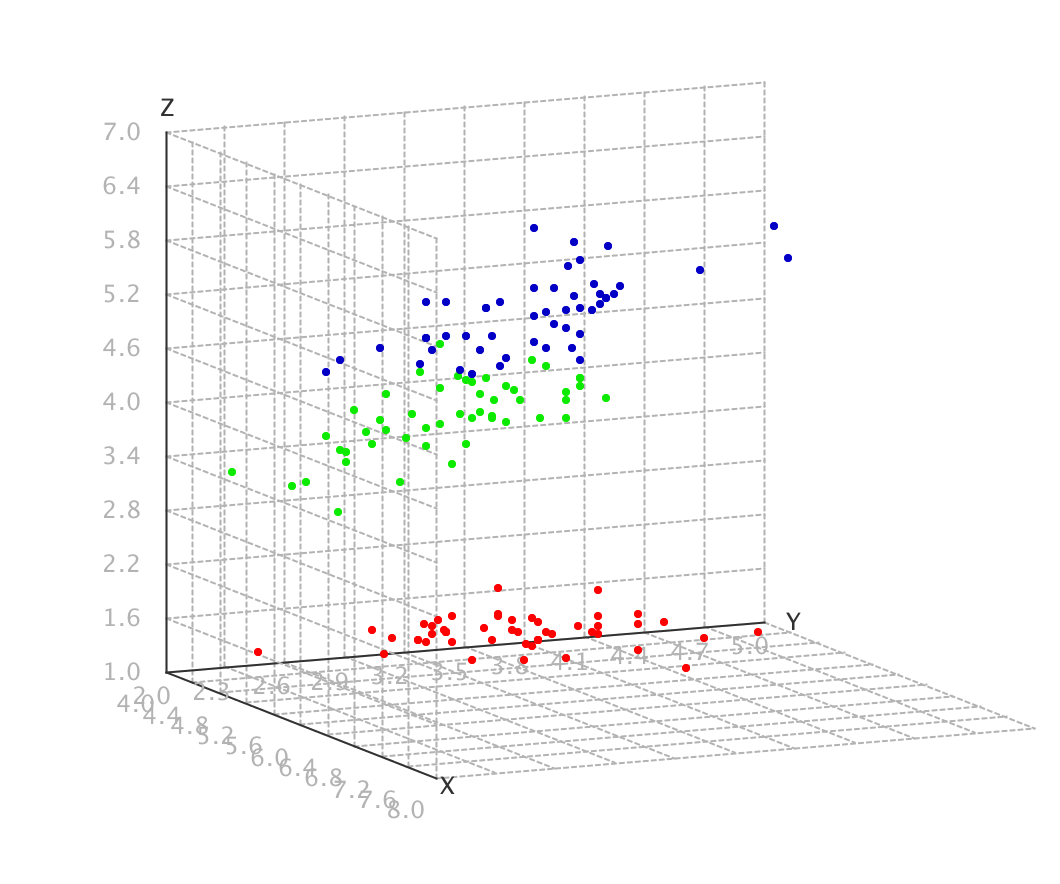
\includegraphics[scale=0.35]{scatter.png}}
\newline
{\scriptsize  
Text explaining diagram if needed
}
\captionsetup{font=small}
\captionsetup{width=14cm}
\caption{Scatter plot for Irish dataset}
\label{chpt2:scatterIris}
\end{figure} 


